% ----------------------------------------------------------
\chapter{Ordinary Differential Equations}\label{ch:ode}
% ----------------------------------------------------------

Differential equations came to be together with the invention of calculus.
In fact, they were studied by both Newton and Leibniz, and by many of the greatest mathematicians such as Euler and Bernoulli.
Even when limited to \gls{ODE}s, it would be unreasonable to assume that one chapter of a bachelor thesis could cover what many authors have dedicated entire books to communicate.
Therefore, it is assumed that the reader has a basic (undergraduate level) understanding of the theory of differential equations\footnotemark.
\footnotetext{Otherwise, the books of \textcite{zill_first_2013} and \textcite{simmons_differential_2017} are great resources.}

This first chapter is, then, a short review of \gls{ODE}s and how to solve them numerically.
This way, the focus is on reviewing the fundamentals and establishing a notation concise for the following chapters.
Furthermore, the approach to numerically solve \gls{ODE}s and the Van der Pol oscillator are also introduced, as they are essential for the experiments described in Chapter \ref{ch:experiments}.

\section{Introduction and Definitions}

A differential equation can be seen as a description of the relationship between unknown quantities and their rates of changes.
Because of this broader definition and direct relationship to applications, differential equations arise naturally in many fields of applied sciences \cite{hairer_solving_1993}, as it is often the case that the rate of change of a certain quantity of interest is related to the rate of change of other quantities.
A classical example of a differential equation is Newton's second law of motion, 
\begin{equation}
   F\left( x\left( t \right) \right) = M \frac{d^2}{d t^2} x(t) \label{eq:newton}
,\end{equation}
in which $x\left( t \right) $ is the position of an object at time $t$, $M$ is its mass, and $F(x)$ is the force under which the object is at a given position.
This example highlights one of the great powers of the differential equations, which is to describe the dynamics of a certain phenomenon without explicitly defining it.


For a more tangible definition, any equation that contains the derivatives of (at least) one unknown function with respect to (at least) one independent variable is called a \emph{differential equation} \cite{zill_first_2013}.
A differential equation that involves only \emph{ordinary} derivatives, that is, only derivatives of functions with respect to a single variable, (such as the one above) is called an \gls{ODE}.
% A differential equation can also be classified through its \emph{order} (the order of its highest derivative)
\gls{ODE}s can be represented in the normal form \[
    \frac{d^n \bm{x}(t)}{d t^{n}} = \mathcal{N}'\left( t, \bm{x}\left( t \right), \frac{d \bm{x}(t)}{d t}, \ldots,\frac{d^{n-1}\bm{x}(t)}{d t^{n-1}} \right)
.\] 
in which $\bm{x}:\R\to \R^{m'} $, $\mathcal{N}':\R\times \R^{nm'}\to \R^{m'}$ is a continuous function, $\frac{d^n \bm{x}(t)}{d t^{n}}$ is the vector containing the derivatives with respect to $t$ of all $\bm{x}\left( t \right) $ components\footnotetext{I.e., the first (and only) row-vector of the Jacobian of $\bm{x}\left( t \right) $.}, and $n$ is the order of the highest derivative in the equation and is commonly referred to as the \emph{order of the differential equation}.

Any function $\bm{\phi}:I\subset\R\to \R^{m'}$, $I$ an interval, is said to be a \emph{solution} of an $n$-th order \gls{ODE} if it is $n$-times differentiable on $I$ and it satisfies
\[
    \frac{d^n \bm{\phi}(t)}{d t^{n}} = \mathcal{N}'\left( t, \bm{\phi}\left( t \right) , \frac{d \bm{\phi}(t)}{d t}, \ldots,\frac{d^{n-1}\bm{\phi}(t)}{d t^{n-1}} \right),\,\forall t\in I
.\]
Note, however, that the solutions are not necessarily unique.
As an example, given Newton's second law of motion, as shown in equation \eqref{eq:newton}, with constant force ($F(x)=C$), then it is easy to see that any second-order polynomial of the form:
\[
    \phi\left( t \right) = \frac{C}{2M}t^2 + a_1t + a_0,\, a_0,a_1\in \R
\]
is a solution.

Now, given an $n$-th order \gls{ODE}, let $\bm{y}_1\left( t \right) =\bm{x}\left( t \right),\,\bm{y}_2\left( t \right) = \frac{d \bm{x}\left( t \right) }{d t} ,\ldots, \bm{y}_n\left( t \right) = \frac{d^{n-1} \bm{x}\left( t \right) }{d t^{n-1}}$.
Note that we can now write the following \emph{system} of first-order differential equations:
\begin{align*}
    \frac{d \bm{y_1}\left( t \right) }{dt} &= \frac{d \bm{x}\left( t \right) }{d t} = \bm{y}_2\left( t \right) \\
    &~~\vdots \\
    \frac{d \bm{y_{n-1}}\left( t \right) }{dt} &= \frac{d^{n-1} \bm{x}\left( t \right) }{d t^{n-1}} = \bm{y}_n\left( t \right) \\
    \frac{d \bm{y_n}\left( t \right) }{dt} &= \frac{d^{n} \bm{x}\left( t \right) }{d t^{n}} = \mathcal{N}'\left( t, \bm{x}\left( t \right), \frac{d \bm{x}(t)}{d t}, \ldots,\frac{d^{n-1}\bm{x}(t)}{d t^{n-1}} \right) = \mathcal{N}'\left( t, \bm{y}_1\left( t \right), \ldots, \bm{y}_n\left( t \right) \right)
.\end{align*}
Then, for $m=n m'$, define $\bm{y}:\R\to \R^{m}$ such that \[
\bm{y}\left( t \right)  = \begin{bmatrix} 
\bm{y}_1\left( t \right) \\ \vdots \\ \bm{y}_n\left( t \right) 
\end{bmatrix} 
,\] and $\mathcal{N}:\R\times \R^{m}\to \R^{m}$ such that \[
    \mathcal{N}\left( t,\bm{y}\left( t \right)  \right) = \begin{bmatrix} 
    \bm{y}_2 \\ \vdots \\ \bm{y}_n \\ \mathcal{N}'\left( t, \bm{y}_1\left( t \right), \ldots, \bm{y}_n\left( t \right) \right)
    \end{bmatrix} 
.\] With this, it is easy to see that the first-order \gls{ODE}
\begin{equation}\label{eq:ode}
    \frac{d \bm{y}\left( t \right) }{d t} = \mathcal{N}\left( t, \bm{y}\left( t \right)  \right) 
\end{equation}
is equivalent to the original $n$-th order \gls{ODE}, that is, given a solution for one of the equations, one can trivially derive the solution for the other.
This allows us to focus on first-order \gls{ODE}s for the remaining of the chapter.

Let us take once again Newton's second law (eq. \eqref{eq:newton}) with constant force $F(x)=C$.
This equation in the normal form can be written
\[
    \frac{d^2 x\left( t \right) }{dt^2} = \frac{C}{M}
.\] 
Now, define $\bm{y}:\R\to \R^2$, $\bm{y}(t) = \left( y_1\left( t \right) ,y_2\left( t \right)  \right) $ such that $y_1(t) = x(t)$ and $y_2(t)=\frac{d x(t)}{dt}$. 
Thus, we can write the first order \gls{ODE}
\[
    \frac{d \bm{y}\left( t \right) }{dt} = \begin{bmatrix} \frac{d y_1\left( t \right) }{dt} \\ \frac{d y_2\left( t \right) }{dt} \end{bmatrix} = \begin{bmatrix} y_2(t) \\ \frac{C}{M} \end{bmatrix} 
.\]
The solution to this equation is of the form
\[
    \begin{bmatrix} \frac{C}{2M}t^2 +a_1t + a_0 \\ \frac{C}{M}t + a_1 \end{bmatrix},\, a_1,a_0 \in \R
,\]
which, from the definition of $\bm{y}(t)$, is in accord to the solution for the original ODE.

\section{Initial Value Problems}

It is a common problem to find an explicit definition of the unknown functions in a differential equation.
For \gls{ODE}s, it is often the case that, if one knowns side conditions on the unknown function, then a solution exists and it is unique.
More precisely, for an \gls{ODE} defined as in \eqref{eq:ode}, conditions of the form \[
   \bm{y}\left( t_0 \right) =\bm{y}_0
\] guarantee the existence and uniqueness of an (analytic) solution in the interval $I\subset \R$, $t_0\in I$, if $\mathcal{N}$ is an analytic function\footnotemark\, in $I\times R$, $R\subset \R^m$ with $\bm{y}_0\in R$, guarantee the existence and uniqueness of an (analytic) solution in $I$ if $\mathcal{N}$ is an analytic function\footnotemark in $I\times R$, which is the case for many practical applications \cite{iserles_first_2008}.
\footnotetext{A function is said analytic if and only if its Taylor series expansion converges in the entirety of its domain.}
The problem of finding the solution given conditions as above is called the \gls{IVP}.

\gls{IVP} shows up frequently when the current (or past) state of a system is known and the future state is desired.
Recalling Newton's second law example, suppose that, besides $F(x)=C$, it is also known that the object lies still at $t=0$, i.e., \[
y(0) = 0,\,\frac{d y(0)}{dt}=0
,\] and we are interested in the solution in the interval $I=\left[ 0,T \right] $, for $T>0$. Then, the only solution is that with $a_0=a_1=0$, that is, \[
    \phi\left( t \right) = \frac{C}{2M}t^2
.\] 

\section{Numerical Solvers}

\subsection{Euler's Method}

In an \gls{IVP}, one effectively has the value of $\bm{y}\left( t \right) $ at a given instant in time $t_0$ and can find the slope at that time through $\mathcal{N}$.
Therefore, it is natural that an efficient numerical solution is derived from the linear approximation of $\bm{y}\left( t \right) $ at $t_0$.
In practice, this means to approximate $\mathcal{N}\left( t, \bm{y}\left( t \right) \right) \approx \mathcal{N}\left( t_0, \bm{y}_0 \right),\,\forall t\in I^h $, where $I^h$ is a neighborhood of $t_0$ (i.e., $I^h \subset I$ is an interval with length $h$ such that $t_0\in I^h$).
Then, the approximate solution is
\begin{align*}
    \bm{\phi}\left( t \right) &= \bm{y}\left( t_0 \right) + \int_{t_0}^{t}\mathcal{N}\left( \tau, \bm{y}\left( \tau \right) \right)d\tau \\
    &\approx \bm{y}\left( t_0 \right) + \left( t-t_0 \right)\mathcal{N}\left( t_0, \bm{y}_0 \right),\,t\in I^h
.\end{align*}

Of course, the performance of this naïve approach (for any non-constant $\mathcal{N}$) is satisfactory only for small $h$.
However, one can perform many of such approximations with arbitrarily small $h$.
Let us assume that $I=\left[ t_0,t_N \right]$\footnotemark\, and that one desires an approximation of an exact solution $\bm{\phi}\left( t \right) $ on $I$.
\footnotetext{If $t_0$ is not the extrema of the interval, one can just apply the method in both directions.}
Given a sequence $t_0,\ldots,t_i,\ldots,t_N$ such that $t_{i+1}-t_i=h,\,i=1,\ldots,N$, let us call $\bm{y}_{i}$ the approximation of an exact solution at $t_i$ for $i=1,\ldots,N$, i.e., $\bm{y}_{i}\approx \bm{\phi}(t_i)$.
One can use the first order approximation recursively to compute \[
\bm{y}_{i+1} = \bm{y}_{i} + h\mathcal{N}\left( t_i, \bm{y}_i \right),\,i=1,\ldots,N
\] with (theoretically) arbitrary precision \cite{iserles_first_2008}.
This is true because $\|\bm{y}_{i+1}-\bm{\phi}(t_{i+1})\|$ is related to the size of the \textit{time step} $h$.
This approach is the \emph{Euler's method}, and besides being the most simple way of effectively solving the \gls{IVP}, it forms the basis of most of the commonly used advanced numerical solvers for \gls{ODE}s.

\subsection{Runge-Kutta Method}

Euler's method comes short in that it uses \emph{only} the information from the previous step at each iteration, i.e., it discards the information from the previous steps.
The \emph{Runge-Kutta methods}, on the other hand, feeds from the rich theory on numerical integration and uses multiple approximations of $\bm{y}\left( t \right)$ to take a step.
More precisely, the \gls{RK4} uses 4 approximations of the solution to estimate $\bm{y}_{i+1}$.

Similar to Euler's method, Runge-Kutta is also an iterative approach, which means that given $\bm{y}_i$ (an approximation of the solution at $t_i$) it will compute $\bm{y}_{i+1}$ (an approximation of the solution at $t_{i+1}=t_i + h$).
The intuition of \gls{RK4} is to iteratively approximate $\mathcal{N}$ (the slope) for the solution \emph{within} the step (i.e, the interval $\left[ t_i,t_{i+1} \right] $) and use this information to compute $\bm{y}_{i+1}$.
Let us denote $\bm{k}_1,\ldots,\bm{k}_4$ as intermediate approximations of $\mathcal{N}$ such that
\begin{align*}
    \bm{k}_1 &= \mathcal{N}\left( t_i , \bm{y}_i \right)  \\
    \bm{k}_2 &= \mathcal{N}\left( t_i+\frac{h}{2}, \bm{y}_i + \frac{h}{2}\bm{k}_1 \right)  \\
    \bm{k}_3 &= \mathcal{N}\left( t_i+\frac{h}{2}, \bm{y}_i + \frac{h}{2}\bm{k}_2 \right)  \\
    \bm{k}_4 &= \mathcal{N}\left( t_i+h, \bm{y}_i + h \bm{k}_3 \right)
.\end{align*}
Note that each approximation depends on the previous ones, being computed in sequence.
Furthermore, one can see that $\bm{k}_1$ is the approximation of $\mathcal{N}$ at the beginning of the step ($t_i$ ), while $\bm{k}_2$ and $\bm{k}_3$ are at the middle and $\bm{k}_4$ is at the end ($t_{i+1}$).
Finally, $\bm{y}_{i+1}$ is computed taking a weighted average of these approximations as \[
    \bm{y}_{i+1} = \bm{y}_i + h \frac{\bm{k}_1 + 2\bm{k}_2 + 2 \bm{k}_3 + \bm{k}_4}{6}
.\]

Even though Runge-Kutta's approach seems quite simple and magic, it provides a significant error reduction in a still very lean algorithm.
In fact, even when one bases around the number of evaluations of the $\mathcal{N}$ function (which tends to be the costlier operations for more complex functions), it still outperforms the Euler's method, even with a step size 5 times larger\footnotemark.
\footnotetext{Each iteration of \gls{RK4} makes 5 $\mathcal{N}$ function evaluations while Euler's method's makes only one evaluation for iteration, so we can estimate that \gls{RK4} is 5 times more expensive than Euler's.}
This combination makes \gls{RK4} one of the most used ODE solvers yet.
An example can be seen in Figure \ref{fig:ode_comparison}.

\begin{figure}[h]
    \centering
    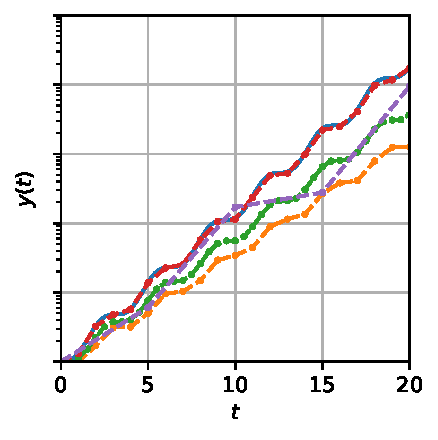
\includegraphics{images/ode_solver_comparison_zoom.pdf}
    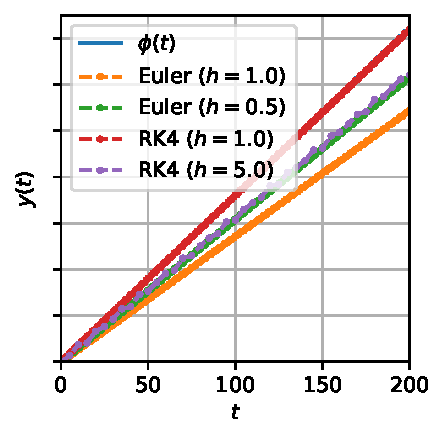
\includegraphics{images/ode_solver_comparison.pdf}
    \caption{Comparison of \gls{RK4} and Euler's method for $\frac{d y\left( t \right) }{dt} = y(t)\sin(t)^2$ with $y(0)=1$. The analytical solution $\phi(t)$ is shown in the solid line while the solvers with different step sizes are shown in broken lines. The image on the right shows the impact in a long-term run, highlighting the comparison between \gls{RK4} with $h=5$ and Euler's with $h=1$.}
    \label{fig:ode_comparison}
\end{figure}

\section{Van der Pol Oscillator}

The Van der Pol oscillator was first described in \textcite{van_der_pol_theory_1920} on the study of oscillatory behavior in electrical circuits with triodes.
Since then, it has been used plenty to model natural phenomena \cite{lucero_modeling_2013,fitzhugh_impulses_1961,nagumo_active_1962,cartwright_dynamics_1999}.
A common representation is as a second-order differential equation \[
    \frac{d^2 y(t)}{dt^2} = \mu\left( 1-y(t)^2 \right) \frac{d y(t)}{dt} + y(t)
,\] 
where $\mu\in \R$ dictates the \emph{dampening} behavior. 
As has been shown in the previous section, the equation can be written in the form of equation \eqref{eq:ode} as
\begin{equation}\label{eq:vdp}
    \frac{d}{dt}\begin{bmatrix} y_1\left( t \right) \\ y_2\left( t \right)  \end{bmatrix} = \begin{bmatrix} 
y_2\left( t \right) \\
\mu\left( 1-y_1\left( t \right) ^2 \right) y_2\left( t \right) - y_1(t)
\end{bmatrix} 
.\end{equation}
In the example shown in Figure \ref{fig:vdp_example}, the impact of $\mu$ in the non-linearity of the solution is shown.

The Van der Pol oscillator has no analytic solution \cite{panayotounakos_lack_2003}, so it requires an accompanying numerical solver to be studied.
Nevertheless, it is well known that the oscillator has a unique and stable \emph{limit cycle}\footnotemark \cite{grimshaw_nonlinear_1993}. 
\footnotetext{Loosely defined, a limit cycle can be seen as the image of the solution when it becomes periodic. Refer to \textcite{grimshaw_nonlinear_1993} for a more precise definition.}
These limit cycles can be seen in the examples shown in Figure \ref{fig:vdp_statespace}.

\begin{figure}[h]
    \centering
    \begin{subfigure}[b]{\textwidth}
        \centering
	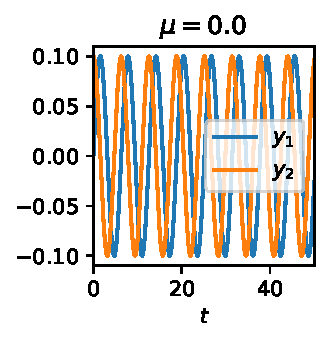
\includegraphics{images/vdp_timeplot_mu_00.pdf}
	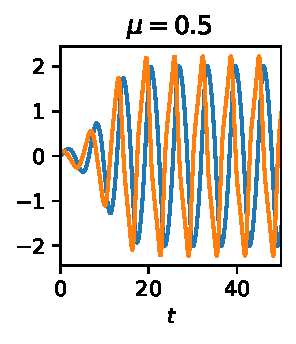
\includegraphics{images/vdp_timeplot_mu_05.pdf}
	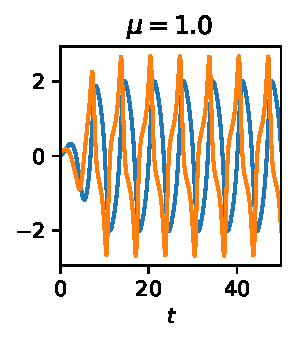
\includegraphics{images/vdp_timeplot_mu_10.pdf}
	\caption{Time evolution}\label{fig:vdp_timeplots}
    \end{subfigure}
    \begin{subfigure}[b]{\textwidth}
        \centering
	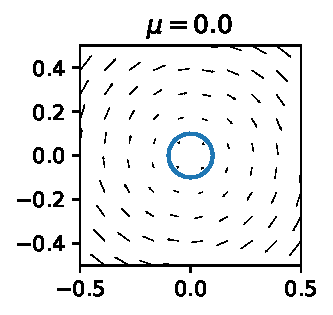
\includegraphics{images/vdp_statespace_mu_00.pdf}
	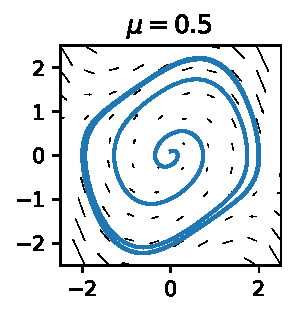
\includegraphics{images/vdp_statespace_mu_05.pdf}
	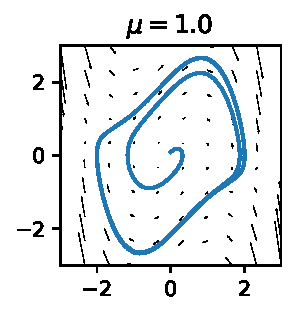
\includegraphics{images/vdp_statespace_mu_10.pdf}
	\caption{State-space}\label{fig:vdp_statespace}
    \end{subfigure}
    \caption{Examples of (numerical) solutions for the Van der Pol oscillator (following Equation \eqref{eq:vdp}) for different values of the dampening parameter but with the same initial condition $y_1(0)=0,\,y_2(0)=0.1$. In (a), the evolution of the numerical solution over 50 seconds is shown. In (b), the trajectory of the numerical solution ($y_2$ in the vertical axis and $y_1$ in the horizontal axis, i.e., a state-space plot) is shown for the same time horizon.}\label{fig:vdp_example}
\end{figure}

